\documentclass{article}
\usepackage[a4paper, margin = 2cm]{geometry}
\usepackage[utf8]{inputenc}
\usepackage[french]{babel}
\usepackage{amssymb}
\usepackage{amsmath}
\usepackage{mathrsfs}
\usepackage{mathtools}
\usepackage{siunitx}
\usepackage{array}
\usepackage{tabularray}
\usepackage{graphicx}
\usepackage[table,xcdraw]{xcolor}
\usepackage{subfigure}
\usepackage{float}
% \usepackage{color}
\usepackage{chngcntr}
\counterwithin{figure}{section}
\counterwithin{table}{section}
\usepackage[hidelinks]{hyperref}
\usepackage{url}
\usepackage{colortbl}
\usepackage{multirow}
\usepackage[dvipsnames]{xcolor}
\usepackage{longtable}
\usepackage{caption}
\usepackage{subcaption}
\usepackage[backend=biber,style=numeric,citestyle=numeric]{biblatex}
\addbibresource{biblio.bib}



\setlength{\parindent}{0pt}

\DeclareSIUnit\msm{m.s.m.}
\DeclareSIUnit\jour{j}
\DeclareSIUnit\mois{mois}
\DeclareSIUnit\an{an}
\DeclareSIUnit\eur{EUR}
\DeclareSIUnit\M{mio}

\begin{document}


\begin{figure}
    \centering
    
\includegraphics[width=0.3\textwidth]{LOGO.png}
\end{figure}

\begin{center}

    \textsc{ \Large CIVIL 466 - Water resources engineering and management}\\[0.5cm]
    \begin{figure}[H]
    \centering
    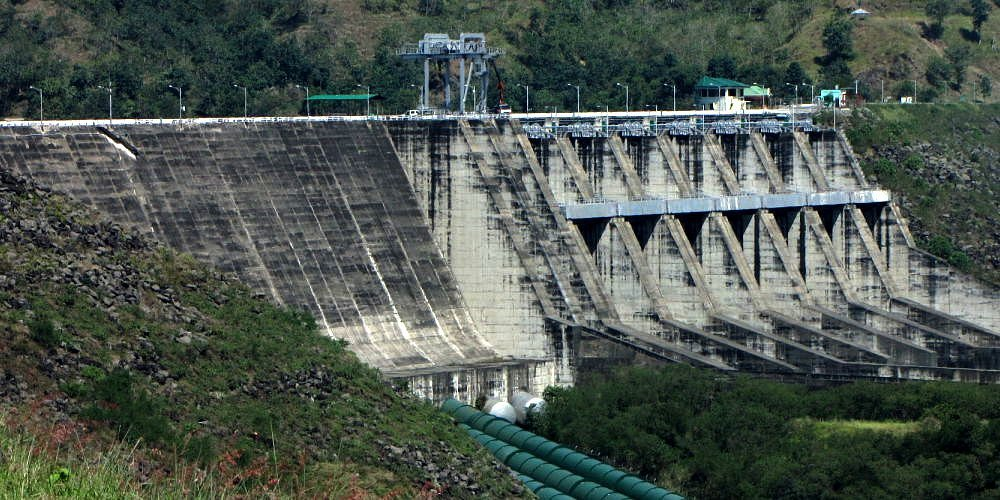
\includegraphics[width=0.8\textwidth]{magat-damm-isabela.jpg}
    \end{figure}
    \vspace{0.3cm}
    \hrule
    \vspace{0.5cm}
    {\Huge \bfseries Practical Work : Case study - Hydropower optimal water allocation and financial study}
    
    
    \vspace{0.5cm}
    
    {\huge \centering \Large Spring 2024}
    
    \vspace{0.5cm}
    \hrule

    \vspace{0.5cm}

    \emph{\Large \centering Groupe 2:}\\
    \vspace{0.5cm}
    \large Moea \textsc{\large Geffard Lemaître}\\
    \large Matteo \textsc{\large Thomé}\\
    \large Pierre \textsc{\large Demey}\\
    \large Margaux \textsc{\large Cochard}\\


    \vspace{0.5cm}

    \emph{\Large \centering Supervisors:}\\
    \vspace{0.5cm}
    \large Junjia   \textsc{\large Kang}\\
    \large Giulio   \textsc{\large Calvani}\\
\end{center}

\newpage

\section{Introduction}
\newpage
\section{Gross water need}

\subsection{Irrigation net water need}

The mass balance equation relates the water stock variation with incomes and outcomes:

\[
\Delta S = Q_{in} - Q_{out} =  P - Q - Irr - ET
\]

Neglecting losses nor interception during precipitation and considering the reserve 





\section{Optimal water allocation}

\begin{figure}
    \centering
    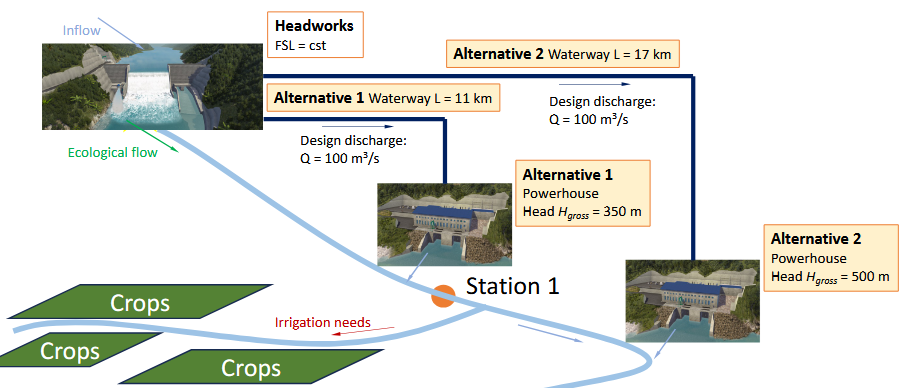
\includegraphics[width=0.8\textwidth]{images/alternatives_schema.png}
    \caption{Diagram presenting the two alternatives.}
    \label{fig:water-allocation}
\end{figure}

In this part, we will perform numerical simulations to assess two project alternatives from both ecological and energetic efficiency standpoints. The objective is to construct the Pareto frontier and evaluate the proposed allocations based on their proximity to this frontier. This analysis will be conducted for each project alternative individually, resulting in two separate simulations, and will account for both wet and dry year periods.





\end{document}